% Capability cliff: per-task mean composite score vs GT file count (log scale).
% Data: reports/eval_scores_v2_long.csv, base_repo/*/eval/gt_files.txt.
% Generated by gen_cliff_data.py.
\begin{figure}[t]
\centering
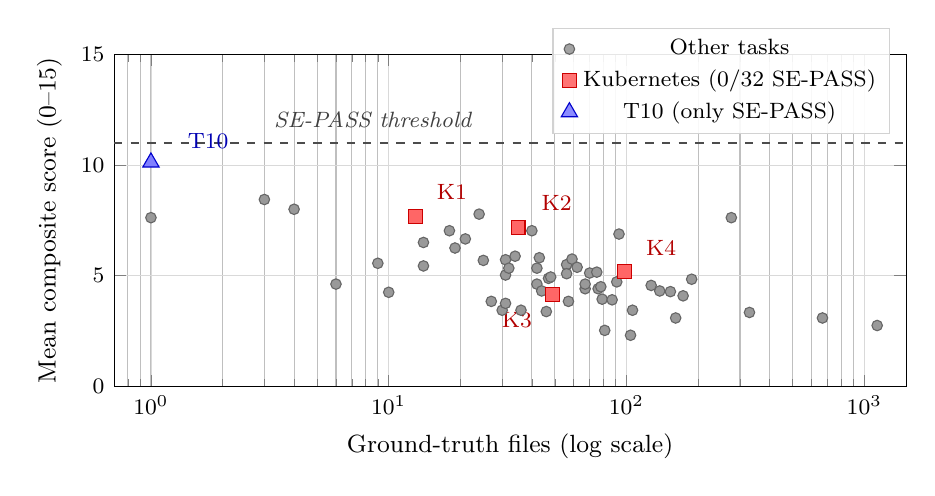
\begin{tikzpicture}
\begin{axis}[
  width=0.96\linewidth,
  height=5.8cm,
  xmode=log,
  log basis x=10,
  xlabel={\small Ground-truth files (log scale)},
  ylabel={\small Mean composite score (0--15)},
  xmin=0.7, xmax=1500,
  ymin=0, ymax=15,
  grid=both,
  major grid style={line width=0.2pt, draw=gray!30},
  minor tick num=0,
  tick label style={font=\footnotesize},
  label style={font=\small},
  legend style={font=\footnotesize, at={(0.98,1.08)}, anchor=north east, draw=gray!35, fill=white, fill opacity=0.9, text opacity=1},
  scatter/classes={
    normal={mark=*, mark size=1.9pt, draw=black!60, fill=black!40},
    kube={mark=square*, mark size=2.5pt, draw=red!80!black, fill=red!60},
    t10={mark=triangle*, mark size=3.4pt, draw=blue!80!black, fill=blue!50}
  },
]

% Regular tasks (calibration C/M + LongBench, excluding K and T10)
\addplot[scatter, only marks, scatter src=explicit symbolic]
  coordinates {
    (1,7.62) [normal]
    (3,8.44) [normal]
    (4,8.00) [normal]
    (6,4.62) [normal]
    (9,5.56) [normal]
    (10,4.25) [normal]
    (14,6.50) [normal]
    (14,5.44) [normal]
    (18,7.03) [normal]
    (19,6.25) [normal]
    (21,6.66) [normal]
    (24,7.78) [normal]
    (25,5.69) [normal]
    (27,3.84) [normal]
    (30,3.44) [normal]
    (31,5.03) [normal]
    (31,3.75) [normal]
    (31,5.72) [normal]
    (32,5.34) [normal]
    (34,5.88) [normal]
    (36,3.44) [normal]
    (40,7.03) [normal]
    (42,5.34) [normal]
    (42,4.62) [normal]
    (43,5.81) [normal]
    (44,4.31) [normal]
    (46,3.38) [normal]
    (47,4.88) [normal]
    (48,4.94) [normal]
    (56,5.50) [normal]
    (56,5.09) [normal]
    (57,3.84) [normal]
    (59,5.75) [normal]
    (62,5.38) [normal]
    (67,4.41) [normal]
    (67,4.62) [normal]
    (70,5.12) [normal]
    (75,5.16) [normal]
    (76,4.41) [normal]
    (78,4.50) [normal]
    (79,3.94) [normal]
    (81,2.53) [normal]
    (87,3.91) [normal]
    (91,4.72) [normal]
    (93,6.88) [normal]
    (104,2.31) [normal]
    (106,3.44) [normal]
    (127,4.56) [normal]
    (138,4.31) [normal]
    (153,4.28) [normal]
    (161,3.09) [normal]
    (173,4.09) [normal]
    (188,4.84) [normal]
    (276,7.62) [normal]
    (329,3.34) [normal]
    (667,3.09) [normal]
    (1133,2.75) [normal]
  };

% Kubernetes tasks
\addplot[scatter, only marks, scatter src=explicit symbolic]
  coordinates {
    (13,7.66) [kube]
    (35,7.19) [kube]
    (49,4.16) [kube]
    (98,5.19) [kube]
  };

% T10 (only main-corpus SE-PASS)
\addplot[scatter, only marks, scatter src=explicit symbolic]
  coordinates {
    (1,10.12) [t10]
  };

% SE-PASS threshold line (A>=4, B>=4, C>=3 => sum >= 11)
\addplot[dashed, black!70, line width=0.9pt, domain=0.7:1500, samples=2] {11};

% Annotations
\node[font=\footnotesize, blue!70!black, anchor=south west] at (axis cs:1.3,10.3) {T10};
\node[font=\footnotesize, black!75, anchor=south west] at (axis cs:3,11.25) {\emph{SE-PASS threshold}};
\node[font=\footnotesize, red!70!black, anchor=south west] at (axis cs:14.5,7.98) {K1};
\node[font=\footnotesize, red!70!black, anchor=south west] at (axis cs:40,7.48) {K2};
\node[font=\footnotesize, red!70!black, anchor=north east] at (axis cs:44,3.78) {K3};
\node[font=\footnotesize, red!70!black, anchor=south west] at (axis cs:110,5.46) {K4};

\legend{Other tasks, Kubernetes (0/32 SE-PASS), T10 (only SE-PASS)}
\end{axis}
\end{tikzpicture}
\caption{Capability cliff. Each point is one task; the $y$-value is the mean composite score averaged across all 8 runs (4~agents $\times$ 2~prompts) and 4~evaluators. The dashed line marks the approximate SE-PASS threshold ($A{+}B{+}C \ge 11$). Only T10 (1~GT file, blue triangle) exceeds the threshold among main-corpus tasks. Kubernetes tasks (red squares) all fall well below despite K1--K2 having moderate GT file counts, illustrating the ``Kubernetes cliff'' where cross-module coordination demands defeat all agents regardless of task size.}
\label{fig:capability-cliff}
\end{figure}
